% RESULTADOS-------------------------------------------------------------------

\chapter{RESULTADOS OBTIDOS}
\label{resultados-obtidos}

Apresentar de forma clara os resultados/benefícios alcançados dentro da empresa, ou pelos clientes atendidos por ela, por meio do trabalho realizado pelo aluno no estágio curricular. Sempre que possível utilizar tabelas e gráficos para facilitar a compreensão \cite{marquesone2016big}.

	Nesta seção há o exemplo de como devem ser elaboradas as tabelas e ilustrações (desenhos, imagens, esquemas, fluxogramas, fotografias, gráficos, mapas, organogramas, plantas, quadros, retratos, figuras e outros) \cite{Apache2018}.
    
	Uma tabela deve apresentar dados numéricos de modo resumido e é utilizada principalmente para a apresentação de comparações.

\begin{figure}[!htb]
	\centering
	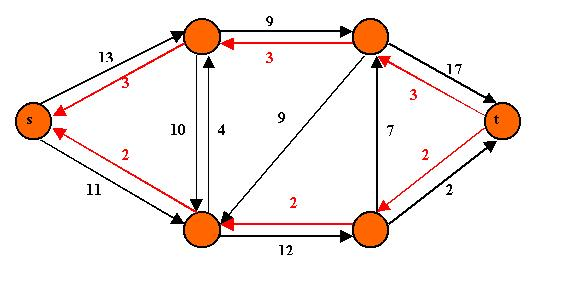
\includegraphics[width=0.9\textwidth]{./figuras/figura1.jpg}
	%	\fonte{\citeonline{IRL2014}}
	\caption{Comunicação entre \textit{cluster}}
	\label{fig:figura1}
\end{figure}